\documentclass[10pt,letterpaper]{article}

\usepackage{psepress}
\addbibresource{refs.bib}

\renewcommand{\PaperTitle}{Explicit Specification Interfaces for Equation-Oriented Process Models: A Pyomo Framework and Agent-Assisted Evaluation}
\renewcommand{\PaperAuthors}{%
Bert Downs\textsuperscript{a*}, Tim Walmsley\textsuperscript{a}}
\renewcommand{\PaperAffiliations}{%
\textsuperscript{a} Ahuora Centre for Smart Energy Systems, University of Waikato, Hamilton, New Zealand\\
\textsuperscript{*} Corresponding Author: \href{mailto:bert.downs@waikato.ac.nz}{bert.downs@waikato.ac.nz}}
\renewcommand{\PaperAbstract}{%
Equation-oriented process models expose equations and variables but rarely expose their intended specification choices. Consequently, composing models, changing study intent, and configuring models with software tools depend on implicit modeller knowledge. We present \texttt{pyomo-replace}, a Pyomo/IDAES framework that represents ordinary specifications as Canonical Variables and alternative specifications as tracked Replacements. Activating a Replacement fixes a non-canonical target while releasing its Canonical Variable as a Guess Variable, preserving the baseline specification count and recording the exchange. Specification Categories and a staged initialization contract further make the configuration inspectable and reusable. We demonstrate the framework on a geothermal power-loop flowsheet and evaluate the complete workflow in constrained AI-agent configuration tasks. Across single recorded \texttt{gpt-5.6-terra} sessions, the replacement workflow required less time and fewer failed model executions than direct fixing for geothermal and heat-integration flowsheets. A three-effect milk-evaporator case required fewer executions but not less elapsed time, consistent with its smaller number of Replacements. These proof-of-concept results do not establish general AI performance or numerical robustness; they indicate that explicit specification interfaces can make process models more composable and operable by software clients.}
\renewcommand{\PaperKeywords}{Artificial Intelligence, Equation-Oriented Modelling, Pyomo, Process Modelling, Simulation}
\renewcommand{\PaperCopyrightText}{%
\textcopyright\ 2027 by the authors. Licensed to PSEcommunity.org and PSE Press under the CC-BY-SA 4.0 license.}

\renewcommand{\HeaderArticleType}{Original Research Article}
\renewcommand{\HeaderReviewType}{Peer Reviewed Conference Proceeding}
\renewcommand{\HeaderConference}{FOCAPO-CPC 2027}
\renewcommand{\HeaderLocation}{Tucson, Arizona, USA, 10-14 January 2027}
\renewcommand{\FooterJournalInfo}{Syst Control Trans V:XXXX-YYYY (2027)}
\renewcommand{\FirstPageFooterID}{[DOI\_DoNotChange]}
\renewcommand{\BodyPageFooterID}{[LAPSE\_DoNotChange]}

\begin{document}
\psemaketitle

\section{Introduction}
Equation-oriented models (EOMs) provide a common set of first-principles equations for design, performance-rating, and operating studies \cite{shacham1982equation,biegler2010nonlinear}. Algebraic modelling languages (AMLs), including Pyomo, and process-model libraries such as IDAES make these models composable from reusable blocks \cite{hart2011pyomo,lee2021idaes}. However, their variables and equations do not usually state which variables a component author expects a client to specify, or how that choice should change with the study intent.

For example, a pump may be specified by mechanical work in a performance-rating calculation, but by outlet pressure in a measured-condition study. A heat exchanger may be specified by its heat-transfer coefficient in one study and by an outlet thermal condition in another. In a conventional AML workflow, either change is a collection of low-level operations: fix one variable, unfix another, provide initial values, and assess the resulting formulation. The relationship between the physical target and the released quantity is left in scripts, comments, or modeller knowledge.

This is an interface problem rather than only a variable-counting problem. A degree-of-freedom (DoF) diagnostic can identify an under- or over-specified formulation, but cannot say which specification is semantically appropriate to exchange, why it was exchanged, or how the altered model should be initialized. This information is important when components are composed into flowsheets and when graphical clients, workflow tools, or coding agents configure a supplied model.

We present \texttt{pyomo-replace}, a specification-management framework for Pyomo/IDAES EOMs. The framework makes a baseline specification explicit through \emph{Canonical Variables}, and represents an alternative specification as a tracked \emph{Replacement}. The contribution is a software interface and controlled state transition, not a new solver or a claim that a zero DoF count guarantees solvability. We demonstrate the interface on a geothermal power loop and evaluate the complete framework workflow in constrained AI-agent configuration tasks. The evaluation is deliberately narrow: it asks whether the interface makes it easier for one coding agent to specify prepared chemical-process flowsheets.

\section{Specification Interface}
\subsection{Problem Context}
For a model with variables $x$, active equality constraints $c(x)=0$, and fixed variables, a useful operational count is
\begin{equation}
  \operatorname{DoF}_{\mathrm{count}} = n_x - n_c - n_f.
\end{equation}
This count is a valuable assembly diagnostic, but zero counted DoF does not prove independent equations, structural nonsingularity, physical feasibility, or numerical convergence \cite{bunus2001debugging,lee2024model}. Process knowledge, structural diagnostics, scaling, and initialization remain necessary. The framework therefore manages specification bookkeeping while complementing rather than replacing those tools.

The specification task also changes on composition. A variable that must be fixed for an isolated block may be determined by an upstream connection in a flowsheet; unconnected inlets instead require external conditions. The flowsheet author must know the expected specification of each unit, select meaningful study targets, and retain suitable guesses when the configuration changes. Existing initialization procedures are usually written for one expected fixed-variable configuration \cite{SAFDARNEJAD201539,lee2021idaes}.

\subsection{Framework Semantics}
A \emph{Specification} declares that a Canonical Variable, or its active Replacement, supplies one degree of freedom. A Canonical Variable is registered as the ordinary specification for its owning block and is labelled with a \emph{Specification Category}, such as inlet, operation, design, or initial condition. Registration fixes newly registered variables; after flowsheet connections are expanded, unconnected inlet-port variables can also be registered.

A Replacement substitutes a non-canonical variable for one Canonical Variable. Activation fixes the replacement variable and unfixes the Canonical Variable, which becomes a \emph{Guess Variable}: it retains a value for initialization but is no longer fixed during the requested solve. Table~\ref{tab:concepts} summarizes the visible contract. This one-for-one exchange preserves the baseline number of fixed Specifications, not a proof that the new specification is suitable.

\begin{table}[htp!]
  \caption{Core elements of the explicit specification interface.}
  \label{tab:concepts}
  \centering
  \renewcommand{\arraystretch}{1.05}
  \begin{tabularx}{\columnwidth}{@{}lX@{}}
    \toprule
    \textbf{Element} & \textbf{Role} \\
    \midrule
    Canonical Variable & Ordinary, fixed specification registered by a block author. \\
    Specification Category & Label for specification intent, such as design or operation. \\
    Replacement & Recorded exchange: a non-canonical variable is fixed and a Canonical Variable is released. \\
    Guess Variable & Released Canonical Variable whose value remains available for initialization. \\
    Replacement Candidate & Unfixed non-canonical variable that may be requested as a Replacement. \\
    \bottomrule
  \end{tabularx}
\end{table}

The authoritative state is attached to the flowsheet, allowing a Replacement to span block boundaries while retaining one record. The implementation requires both variables to be contained by that flowsheet; the released variable to be a currently fixed Canonical Variable; and the replacement to be a wholly unfixed, non-canonical variable. It treats indexed variables atomically, rejecting partially fixed indexed variables. After an exchange, it checks the Pyomo incidence graph and restores the previous state if the Dulmage--Mendelsohn decomposition reports unmatched constraints \cite{bunus2001debugging}.

The client interface is concise:
\begin{lstlisting}[style=psecode]
specs = SpecificationState.for_flowsheet(
    model.fs
)
specs.register([
    (unit.heat_duty, "operation")
])
specs.register_inlet_ports(model.fs)
specs.replace(unit.heat_duty,
              unit.outlet.enth_mol)
\end{lstlisting}
Inspection methods report Canonical Variables, Replacement Candidates, active Replacements, and Guess Variables for a flowsheet or block. A category can be deactivated to undo its associated Replacements, returning the relevant Canonical Variables to their baseline role.

\subsection{Staged Initialization}
The explicit relationship also supports a reusable initialization contract. During initialization, the framework can temporarily suspend the relevant Replacements: Canonical Variables are fixed and replacement variables are released. A unit or flowsheet is initialized in this expected baseline configuration, then the requested Replacements are restored and the model is solved again. This lets the released Canonical Variable supply a retained guess without requiring each unit initializer to enumerate every valid alternative specification. It remains a workflow convention, not a convergence guarantee.

\section{Geothermal Demonstration}
The main demonstration is a steady-state geothermal-heated $n$-butane power loop comprising a pump, turbine, recuperator, preheater, vaporizer, condenser, water mixer, and recycle. It uses Helmholtz property packages for water and $n$-butane. Heat exchangers register overall heat-transfer coefficient and area as design Canonical Variables; pumps and turbines register mechanical work as an operation Canonical Variable and efficiency as a design Canonical Variable. Unconnected inlet-port variables are registered after the arcs are expanded.

\begin{figure}[htp!]
  \centering
  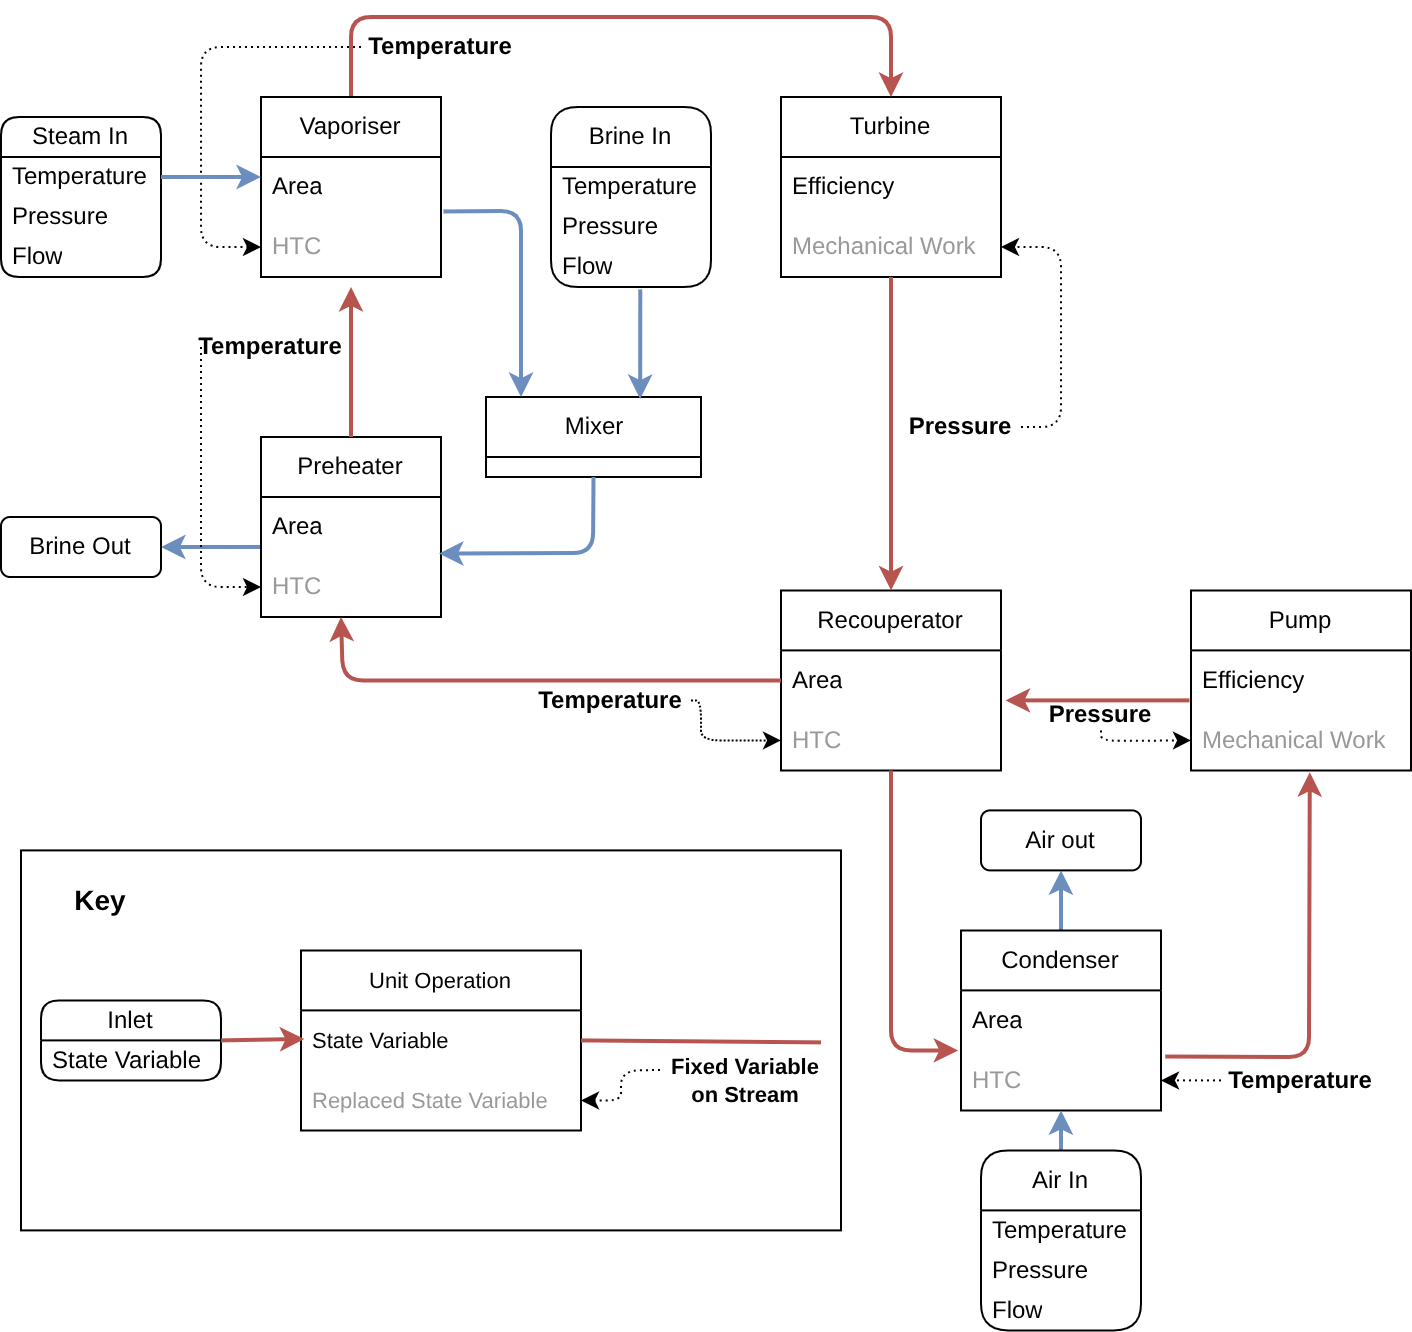
\includegraphics[width=\columnwidth]{../../paper/assets/geothermal-replacement.drawio.png}
  \caption{Geothermal power-loop example. A study target can replace a baseline Canonical Variable while retaining an explicit record of the exchange.}
  \label{fig:geothermal}
\end{figure}

The executable replacement-enabled case fixes a condenser shell outlet temperature of 274.970 K in place of the condenser overall heat-transfer coefficient. The coefficient becomes a Guess Variable. More generally, an outlet enthalpy can replace a heat-transfer coefficient when sizing an exchanger to a thermal target, and an outlet pressure can replace pump or turbine work in an operating study. Figure~\ref{fig:geothermal} illustrates this distinction: the physical target is explicit, while the baseline variable remains available to initialize the subsequent solve.

The recycle is initialized using Pyomo sequential decomposition and tear-stream guesses. The sequence first suspends Replacements, initializes and solves the canonical configuration, restores the requested Replacements, and finally solves the target configuration. This example demonstrates auditable study reconfiguration; it does not imply that all target values are feasible or that all replacements initialize successfully.

\section{Agent-Assisted Configuration Evaluation}
\subsection{Method}
We evaluated whether an explicit specification interface makes a constrained coding task easier for \texttt{gpt-5.6-terra}. Each clean OpenCode session received a Markdown scenario and a Python template with the flowsheet topology, unit operations, arcs, diagnostics, initialization, and solve routines. The agent could edit only \texttt{specify\_model}, was prompted once with no human follow-up, and was asked to run the model until it solved according to the supplied scenario.

The direct template required \texttt{var.fix()} calls. The replacement template exposed Canonical Variables, examples, replacement diagnostics, and the staged initialization contract; it required a Replacement before fixing a non-canonical variable. A second direct condition allowed approximate \texttt{set\_value()} guesses. The experiment therefore compares complete workflows, not the isolated causal effect of replacement metadata. It covers a geothermal power loop, a water-only heat-integration and steam-generation flowsheet, and a three-effect milk evaporator with mechanical-vapor-recompression recycles. The prepared templates constrain the task to specification, rather than open-ended model construction.

We recorded session duration, model executions, failed executions, patches, and tokens from exported sessions. A successful execution was inferred from the recorded non-failed final execution; no independent accuracy metric was calculated. There is one session per condition, so the observations have no uncertainty intervals and should not be treated as a performance distribution.

\subsection{Results}
Table~\ref{tab:results} reports the session-level results. For geothermal, the replacement workflow took 110.5~s, compared with 348.9~s for direct fixing and 385.3~s for direct fixing with guesses. It required two model runs and one failed run, versus five and four in the direct condition. For heat integration, the replacement workflow took 207.4~s versus 378.8~s and 426.5~s, with three runs and two failures versus nine and six in the direct condition.

\begin{table}[!ht]
  \caption{Recorded single-session agent results. Failures include environment and execution failures, not only solver failures.}
  \label{tab:results}
  \centering
  \footnotesize
  \renewcommand{\arraystretch}{1.02}
  \begin{tabular}{@{}llrrr@{}}
    \toprule
    \textbf{Flowsheet} & \textbf{Workflow} & \textbf{Time (s)} & \textbf{Runs} & \textbf{Failures} \\
    \midrule
    Geothermal & Direct & 348.9 & 5 & 4 \\
    Geothermal & Direct + guesses & 385.3 & 10 & 7 \\
    Geothermal & Replacement & 110.5 & 2 & 1 \\
    Heat integration & Direct & 378.8 & 9 & 6 \\
    Heat integration & Direct + guesses & 426.5 & 12 & 11 \\
    Heat integration & Replacement & 207.4 & 3 & 2 \\
    Milk evaporator & Direct & 109.6 & 3 & 2 \\
    Milk evaporator & Direct + guesses & 93.5 & 3 & 2 \\
    Milk evaporator & Replacement & 113.8 & 2 & 1 \\
    \bottomrule
  \end{tabular}
\end{table}

The milk-evaporator case qualifies this pattern. The replacement workflow used one fewer model run and failed run, but took 113.8~s, marginally longer than direct fixing and 20.3~s longer than direct fixing with guesses. It contains only three repeated compressor outlet-pressure Replacements for compressor-work Canonical Variables; much of the scenario is specified identically in all conditions. Thus, it demonstrates that the workflow applies to a coupled multi-domain recycle flowsheet, but provides less opportunity for the interface to reduce the specification-search burden.

Qualitatively, direct workflows required the agent to infer a sufficient set of fixed variables and, for difficult cases, devise initialization guesses. The replacement workflow instead presented a constrained operation: state a scenario-facing target and the Canonical Variable it replaces. The recorded replacement reports preserve this provenance, while staged initialization retains released values as guesses. These features are consistent with the lower iteration observed in the geothermal and heat-integration sessions.

\section{Discussion and Conclusions}
\texttt{pyomo-replace} treats specification intent as an explicit interface for reusable EOM components. Canonical Variables define the baseline contract, categories convey their role, and Replacements record which physical target now supplies a Specification and which Canonical Variable is a Guess Variable. This makes configuration state inspectable by clients without changing the underlying equations or solver.

The agent study provides bounded evidence that this interface can make prepared process models more machine-operable. In the geothermal and heat-integration sessions, the complete replacement workflow was associated with fewer model executions, fewer failures, and shorter session durations. The milk-evaporator result shows that this is not a universal time advantage, especially when a task contains few replacements. The results are not evidence of general AI capability, human usability, or universal numerical robustness.

Several limitations are important. There was one run per condition, one agent model, related prompts, and prepared templates. OpenCode versions varied across cases. The replacement template also includes diagnostics, examples, and staged initialization that are absent from the direct templates, so the comparison cannot isolate metadata from API, prompt, or initialization effects. Some failed runs were environment or interpreter failures rather than numerical failures. Finally, preserving a counted DoF does not establish structural nonsingularity, feasibility, physical validity, or convergence.

Despite these limits, an explicit specification interface provides a useful boundary for process-model libraries and automation tools. It records configuration provenance, supports switching between study intents, and offers a reusable initialization contract. Future work should test independent repetitions, additional agents and model families, and human-facing configuration tools.

\section*{Acknowledgements}
This research was funded by the Ahuora Centre for Smart Energy Systems under the New Zealand Ministry of Business, Innovation and Employment Advanced Energy Platform Technology research programme.

\section*{Data Availability}
A sample implementation of replacement logic in Pyomo, initialization tests, and the geothermal model example are available at \url{https://github.com/bertkdowns/pyomo-replace}.

\section*{Declaration of Use of AI}
Generative AI was used to assist in preparing an initial manuscript draft. The authors are responsible for reviewing, verifying, and revising the manuscript. The AI-agent configuration experiment is described in the main text.

\pseprintreferences
\pseprintcopyright
\end{document}
